\documentclass[11pt]{article}
%AMS-TeX packages
\usepackage{graphicx}
\usepackage{amssymb, amsmath, amsthm} 
\usepackage[margin=.75in]{geometry}
\usepackage{graphicx}
\usepackage{bm} % bold math
\usepackage{listings}
\usepackage{color} %red, green, blue, yellow, cyan, magenta, black, white
\definecolor{mygreen}{RGB}{28,172,0} % color values Red, Green, Blue
\definecolor{mylilas}{RGB}{170,55,241}

%Redefining sections as problems
\makeatletter
\newenvironment{problem}[1][\unskip]{\@startsection
       {section} 
       {1}
       {0em}
       {-3.5ex plus -1ex minus -.2ex}
       {0.1ex}
       {\pagebreak[3]\large\bf\noindent{Problem #1 }}  \\}
\makeatother

\newenvironment{argument}[1][\unskip]{%
\@startsection{section}{1}{0em}{-3.5ex plus -1ex minus -.2ex}{0.1ex}
{\noindent\textbf{\large{\bf{Argument #1 }}}}\\
\noindent}
{}

%Fancy-header package to modify header/page numbering 
\usepackage{fancyhdr}
\pagestyle{fancy}
\lhead{\textbf{Ge/ESE 118}} %name of the course
\chead{\textbf{}} %topic of the homework set
\rhead{\textbf{Solution 3}} %number of the homework set

%%% CONTENTS OF THE HW SET %%%
\begin{document}
\lstset{language=Matlab,%
	  %basicstyle=\color{red},
  breaklines=true,%
  morekeywords={matlab2tikz},
  keywordstyle=\color{blue},%
  morekeywords=[2]{1}, keywordstyle=[2]{\color{black}},
  identifierstyle=\color{black},%}
  stringstyle=\color{mylilas},
  commentstyle=\color{mygreen},%
  showstringspaces=false,%without this there will be a symbol in the places where there is a space
  numbers=left,%
  numberstyle={\tiny \color{black}},% size of the numbers
  numbersep=9pt, % this defines how far the numbers are from the text
  emph=[1]{for,end,break},emphstyle=[1]\color{red}, %some words to emphasise
													  %emph=[2]{word1,word2}, emphstyle=[2]{style},    
}


%Include frequently used commands used for equations
%Fractions
\newcommand\fr[2]{\frac{#1}{#2}} %Regular fraction

%Braces, Brackets, Parentheses, etc.
\newcommand\brcs[1]{\{#1\}} %Braces
\newcommand\brckts[1]{\left[#1\right]} %Brackets
\newcommand\lr[1]{\left(#1\right)} %Parentheses
\newcommand\abs[1]{\Big\lvert#1\Big\rvert} %Absolute value
\newcommand\ltwo[1]{\lVert#1\rVert_2} %L2-norm
\newcommand\linf[1]{\lVert#1\rVert_\infty} %L2-norm

%Linear algebra
\newcommand\tr[1]{\text{tr}\left( \mathbf{#1}\right)} %Trace
\renewcommand\det[1]{\text{det}\left( \mathbf{#1}\right)} %Determinant

%Trigonometric & special functions
\newcommand\sinb[1]{\, \sin\left(#1\right)} %Sine with parentheses: sin(x)
\newcommand\cosb[1]{\, \cos\left(#1\right)} %Cosine with parentheses: cos(x)
\newcommand\tanb[1]{\, \tan\left(#1\right)} %Tangent with parentheses: tan(x)
\newcommand\cotb[1]{\, \cot\left(#1\right)} %Cotangent with parentheses: cot(x)
\newcommand\sinc[1]{\, \text{sinc}\left(#1\right)} %Sinc function: sinc = sin(x)/x

%Calculus
\renewcommand\d[1]{\, \text{d}#1} %Differential for integrals
\newcommand\der[2]{\frac{\text{d}#1}{\text{d}#2}} %Ordinary derivate first order
\newcommand\dder[2]{\frac{\text{d}^2#1}{\text{d}#2^2}} %Ordinary derivate second order
\newcommand\od[3]{\frac{\text{d}^{#3}#1}{\text{d}#2^{#3}}} %Ordinary derivate any order
\newcommand\pder[2]{\frac{\partial#1}{\partial#2}} %Partial derivate first order
\newcommand\pdder[2]{\frac{\partial^2#1}{\partial#2^2}} %Partial derivate second order
\newcommand\pd[3]{\frac{\partial^{#3}#1}{\partial#2^{#3}}} %Partial derivative any order

%Fourier transform
\newcommand\ft[1]{\hat{#1}} %Fourier coefficient

%Probability theory, Statistics
\newcommand\ex[1]{\mathbb{E}\left[#1\right]} %Expectation
\newcommand\pr[1]{\mathbb{P}\left(#1\right)} %Probability
\newcommand\Var[1]{\text{Var}\left(#1\right)} %Variance
\newcommand\Cov[1]{\text{Cov}\left(#1\right)} %Covariance
\newcommand\one{\mathbf{1}} %Unity

%Miscellaneous 
\renewcommand\mod{\text{mod}} %Modulo

%Problems
\section*{Problem 1 - (graded by Toby)}

\subsection*{(a) - 5 points}
The range of $\mathbf{G}$ is defined as the linear combination of $\mathbf{G}$'s column vectors. The dimension of the range of $\mathbf{G}$ is therefore equal to the number of linearly independent column vectors of $\mathbf{G}$. Because $\mathbf{G}$ is an $N$ by $M$ matrix, we have at most $M$ linearly independent columns and the maximum dimension of the range of $\mathbf{G}$ is $M$. The data space is $\mathbb{R}^N$ and thus has dimension $N$. If $N> M$. Hence we have that 
\begin{equation}
\dim (\text{range}(\mathbf{G})) \leq M < N.
\end{equation}
This implies that the range of $\mathbf{G}$ is a subspace of $\mathbb{R}^N$ whose dimension is less than $N$.

\subsection*{(b) - 5 points}
We have that $H_{ij} = \mathbf{g}_i^T\mathbf{g}_j$. The diagonal elements of $\mathbf{H}$ are the squared lengths of the column vectors of $\mathbf{G}$. The off diagonal elements can be nonzero and measure how much the column vectors of $\mathbf{G}$ project onto each other, i.e., what their orientation is with respect to each other. If $\mathbf{G}$ is an orthogonal matrix, then $\mathbf{H}$ is a diagonal matrix. If in addition the column vectors have length 1, $\mathbf{H}$ is the unity matrix as shown in problem 3 of the first homework set. Because 
\begin{equation}
\mathbf{g}_i^T\mathbf{g}_j = \ltwo{\mathbf{g}_i}\ltwo{\mathbf{g}_j}\cos(\angle(\mathbf{g}_i,\mathbf{g}_j)),
\end{equation}
the dot product involves a measure of how much two vectors project onto each other, measured by the cosine factor. As a matter of fact, this is one way of defining the cosine in the first place.

\subsection*{(c) - 5 points}
Similarly, $\mathbf{G}^T\mathbf{d} = \left( \mathbf{g}_1^T \mathbf{d}, \hdots, \mathbf{g}_M^T \mathbf{d} \right)^T$ is a column vector whose elements measure how much $\mathbf{d}$ projects onto the different column vectors $\mathbf{g}_i$ as
\begin{equation}
\mathbf{g}_i^T\mathbf{d} = \ltwo{\mathbf{g}_i}\ltwo{\mathbf{d}}\cos(\angle(\mathbf{g}_i,\mathbf{d})).
\end{equation}

\subsection*{(d) - 5 points}
Using standard notation and what we know from parts (b) and (c), the equation as given on the homework set can be written as
\begin{equation}
\begin{pmatrix}
\mathbf{g}_1^T (m_1\mathbf{g}_1 + \hdots + m_M \mathbf{g}_M)\\
\vdots\\
\mathbf{g}_M^T (m_1\mathbf{g}_1 + \hdots + m_M \mathbf{g}_M)
\end{pmatrix}
=
\begin{pmatrix}
\mathbf{g}_1^T \mathbf{d}\\
\vdots\\
\mathbf{g}_M^T \mathbf{d}
\end{pmatrix}.
\end{equation}
Therefore, the least squares solution to this equation $\mathbf{m}$ implies a vector $m_1\mathbf{g}_1 + \hdots + m_M \mathbf{g}_M$ in the range of $\mathbf{G}$ whose projections onto the column vectors of $\mathbf{G}$ equal the projects of the data vector onto the column vectors of $\mathbf{G}$.

\newpage

\section*{Problem 2 - (graded by Stephen)}

\subsection*{(a) - 5 points}
A silly real life example that demonstrates $\pr{x,y}=\pr{x|y}\pr{y}=\pr{y|x}\pr{x}$ can involve peanut butter and jelly sandwiches.  If we assume the population is sandwiches made in the United States today, then $\pr{x,y}$ is the probability that a given sandwich we pick will be peanut butter and jelly.  We can calculate this probability in two different ways.  The first is by multiplying the probability that the sandwich has jelly on it $\pr{y}$ (These sandwiches may have jelly and other ingredients, just jelly, or they may have peanut butter and jelly) by the probability that given the sandwich has jelly on it, that it will also have just peanut butter $\pr{x,y}$.  Conversely, we can begin with the probability that the sandwich has peanut butter $\pr{x}$ and multiply by the probability that given the sandwich has peanut butter that it will also have just jelly $\pr{y|x}$.  The probability given jelly that the sandwich will have peanut butter is NOT the same as given peanut butter that it will also have jelly (there could be many more possible sandwiches that include peanut butter for example).

\subsection*{(b) - 5 points}
Independence of events $x$ and $y$ implies the $\pr{x,y}=\pr{x}\pr{y}$.  An example of this would be two strangers going to a sporting event.  $\pr{x,y}$ is the probability that both strangers are at the game even though they do not know each other.  If these individuals get to the game independently then we can assume the events x and y are independent.  In this case we can find $\pr{x,y}$ by simply multiplying $\pr{x}$ by $\pr{y}$.  To think about this intuitively we can think that person x goes to the games $1/2$ of the time and person y $1/3$ of the time.  If them going to the games is independent then person x will be at 50 percent of the games.  Person y only goes to 33.3 percent of the games, and because they are not related, will go to 33.3 percent of the games that person x is at.  Thus to find the total percent of games at which both are present, we multiply $1/2$ by $1/3$.

These events would not be independent if person x and person y were friends and attended games together, or if they drove to the games together.

\subsection*{(c) - 5 points}
Expectation for x:
\begin{equation}
\ex{x} = \langle x\rangle = \int_{-\infty}^{\infty} x \frac{1}{\sigma\sqrt{2\pi}}e^{-\frac{x^2}{2\sigma^2}} dx  
\end{equation}
The Gaussian is an even function and x is an odd function.  Because we are integrating their product (an odd function) over a symmetric interval, we will get an answer of 0.  We can also do this explicitly:

\begin{eqnarray*}
\ex{x} = \frac{1}{\sigma\sqrt{2\pi}} \int_{-\infty}^{\infty} x e^{-\frac{x^2}{2\sigma^2}} dx \\
\ex{x} = \frac{1}{\sigma\sqrt{2\pi}} \left(\int_{-\infty}^{0} x e^{-\frac{x^2}{2\sigma^2}} dx + \int_{0}^{\infty} x e^{-\frac{x^2}{2\sigma^2}} dx \right) \\
\ex{x} = \frac{1}{\sigma\sqrt{2\pi}} \left(\left.-\sigma^2e^{-\frac{x^2}{2\sigma^2}}\right|_{-\infty}^{0}+\left.-\sigma^2e^{-\frac{x^2}{2\sigma^2}}\right|_{0}^{\infty}\right) \\
\ex{x} = \frac{1}{\sigma\sqrt{2\pi}} \left(-\sigma^2-0+0+\sigma^2\right) \\
\ex{x} = \frac{1}{\sigma\sqrt{2\pi}} \left(-\sigma^2+\sigma^2\right) \\
\ex{x} = 0
\end{eqnarray*}

Expectation for $x^2$:
\begin{equation}
\ex{x^2} = \langle x^2\rangle = \int_{-\infty}^{\infty} x^2 \frac{1}{\sigma\sqrt{2\pi}}e^{-\frac{x^2}{2\sigma^2}} dx  
\end{equation}
This time the Gaussian is multiplied by an even function, so it will not integrate to 0.

\begin{eqnarray*}
\ex{x} = \frac{1}{\sigma\sqrt{2\pi}} \int_{-\infty}^{\infty} x e^{-\frac{x^2}{2\sigma^2}} dx
\end{eqnarray*}

We can do this integral by parts ($\int udv=uv|-\int vdu$): \\
$u=x$ $du=1$ \\
$dv=xe^{-x^2/{2*\sigma^2}}$ $v=-\sigma^2 e^{-x^2/{2*\sigma^2}}$ \\

\begin{eqnarray*}
\ex{x} = \frac{1}{\sigma\sqrt{2\pi}} \left( \left. -\sigma x e^{-\frac{x^2}{2\sigma^2}}\right|_{-\infty}^{\infty} - \int_{-\infty}^{\infty} -\sigma^2 e^{-\frac{x^2}{2\sigma^2}} dx \right) \\
\end{eqnarray*}

The first term will go to zero because the exponential goes to 0 faster than x increases.

\begin{eqnarray*}
\ex{x} = \frac{1}{\sigma\sqrt{2\pi}} \sigma^2 \int_{-\infty}^{\infty} e^{-\frac{x^2}{2\sigma^2}} dx
\end{eqnarray*}

We can now do a variable substitution $\beta=\frac{x}{\sigma}$ , $d\beta=\frac{1}{\sigma}dx$ , $dx=\sigma d\beta$ to do this integral.  We are now left with the integral given in the problem:

\begin{eqnarray*}
\int_{-\infty}^{\infty} \sigma e^{-\frac{\beta}{2}} d\beta = \sigma \sqrt{2\pi}
\end{eqnarray*}

We are now left with:

\begin{eqnarray*}
\ex{x} = \frac{1}{\sigma\sqrt{2\pi}} \sigma^3 \sqrt{2\pi} = \sigma^2
\end{eqnarray*}

ALTERNATE - An alternative way to do this is by using a sneaky derivative trick:
\begin{eqnarray*}
\ex{x^2} = \langle x^2\rangle = \frac{1}{\sigma\sqrt{2\pi}} \int_{-\infty}^{\infty} x^2 e^{-\frac{x^2}{2\sigma^2}} dx 
\end{eqnarray*}

This looks suspiciously like the derivative of a function with respect to $\frac{1}{2\sigma^2}$.  Thus, we can do a substitution of $\alpha = \frac{1}{2\sigma^2}$ and rewrite our integral like so:

\begin{eqnarray*}
-\frac{d}{d\alpha} \left(\int_{-\infty}^{\infty} e^{-\alpha{x^2}} dx\right) 
\end{eqnarray*}

We can pull out this derivative because $\alpha$ has nothing to do with the integral over x.  (I agree that this is very sneaky).  We already know the answer to the integral on the inside, so we use that and then take the derivative of the answer with respect to $\alpha$.

\begin{eqnarray*}
-\frac{d}{d\alpha} \left(\sqrt{\frac{\pi}{\alpha}}\right) = \frac{1}{2\alpha}\sqrt{\frac{\pi}{\alpha}}
\end{eqnarray*}

Now plug back in for $\alpha$ and simplify (don't forget the prefactor we pulled out of the integral at the start).

\begin{eqnarray*}
\ex{x^2} = \frac{1}{\sigma\sqrt{2\pi}} \left(\frac{2\sigma^2}{2}\right) \sqrt{2 \pi \sigma^2} = \sigma^2
\end{eqnarray*}


\subsection*{(d)}

\subsection*{(d.i) - 5 points}
Instead of having just one Gaussian, we now have two Gaussians due to the fact that one fifth of the time the measurement apparatus adds 1 cm to the measurement. The probability of a length measurement $d_i$ given the mean value is:
\begin{equation}
\pr{d_i|L} = \frac{4}{5}\mathcal{N}(d_i|L,\sigma) + \frac{1}{5}\mathcal{N}(d_i|L+1,\sigma).
\end{equation}

Let's rewrite this in terms of the exponential form of the Gaussian:

\begin{eqnarray*}
\pr{d_i|L} = \frac{4}{5}\frac{c_1}{\sigma\sqrt{2\pi}} e^{-\frac{(d_i-L)^2}{2\sigma^2}} + \frac{1}{5}\frac{c_2}{\sigma\sqrt{2\pi}} e^{-\frac{(d_i-(L+1))^2}{2\sigma^2}}
\end{eqnarray*}

We need to normalize this result so that the integral of this over all data (from $-\infty$ to $\infty$) is 1.

\begin{eqnarray*}
1 = \frac{4}{5}\frac{c_1}{\sigma\sqrt{2\pi}} \int_{-\infty}^{\infty} e^{-\frac{(d_i-L)^2}{2\sigma^2}} dL + \frac{1}{5}\frac{c_2}{\sigma\sqrt{2\pi}} \int_{-\infty}^{\infty} e^{-\frac{(d_i-(L+1))^2}{2\sigma^2}} dL
\end{eqnarray*}

These integrals are the same as what we already solved in part c.  The addition of the $d_i$ doesn't change the outcome of the integral, so we already know that both integrate to $\sqrt{2\pi}\sigma$.  Thus we are left with:

\begin{eqnarray*}
1 = \frac{4}{5}c_1 + \frac{1}{5}c_2
\end{eqnarray*}

Thus, both $c_1$ and $c_2$ are 1 and our distribution is normalized.

\begin{eqnarray*}
\pr{d_i|L} = \frac{4}{5}\frac{1}{\sigma\sqrt{2\pi}} e^{-\frac{(d_i-L)^2}{2\sigma^2}} + \frac{1}{5}\frac{1}{\sigma\sqrt{2\pi}} e^{-\frac{(d_i-(L+1))^2}{2\sigma^2}}
\end{eqnarray*}

See attached plot.

\subsection*{(d.ii) - 5 points}
The probability of $L$ given the data $d_i$ is
\begin{equation}
\pr{L|d_i} = \frac{4}{5}\mathcal{N}(L|d_i,\sigma) + \frac{1}{5}\mathcal{N}(L|d_i-1,\sigma).
\end{equation}

We know from Bayes' Theorem that $\pr{L|d_i} \propto \pr{d_i|L} P(L)$.  In this problem we have no prior guess, so the prior is a constant.  This means that $P(L)$ is a constant and can be eliminated from the proportion.  Thus, in this case $P(L|d_i) = P(d_i|L)$.  However, in order to plot the probability we will need to switch the variables $d_i$ and $L$.  In doing this substitution we must be careful to replace the $(L+1)$ with $(d_i-1)$ because the mean is one fifth of the time 1 cm less than the data point measured.  

\begin{eqnarray*}
\pr{d_i|L} = \frac{4}{5}\frac{1}{\sigma\sqrt{2\pi}} e^{-\frac{(L-d_i)^2}{2\sigma^2}} + \frac{1}{5}\frac{1}{\sigma\sqrt{2\pi}} e^{-\frac{(L-(d_i-1))^2}{2\sigma^2}}
\end{eqnarray*}

This is going to give us a similar plot to part c, but the plot will appear mirrored around the data point (see attached plot).

\subsection*{(d.iii) - 5 points}


Assuming the measurements are independent of each other. First calculate $\pr{d_1,d_2|L} = \pr{d_1|L}\pr{d_2|L}$. Then interpret that as $\pr{L|d_1,d_2}$, i.e., the posterior probability assuming a prior that equals $1$ everywhere. Take the derivative with respect to $L$ and set it zero to find the maximum probability $L_\text{max}$.  However, the product of the probabilities will have 3 local maxima.  Plotting the expression is the easiest way to see where the global maximum is.  If we plot the product of the two probabilities we will find that the graph has 3 peaks $(L~8.3,L~9.25,L~10.2)$.  The maximum should be the peak at about $L~9.25$.

\begin{eqnarray*}
\pr{d_1,d_2|L} = \pr{d_1|L} \pr{d_2|L} \\
\pr{d_1,d_2|L} = \left(\frac{4}{5}\frac{1}{\sigma\sqrt{2\pi}} e^{-\frac{(d_i-L)^2}{2\sigma^2}} + \frac{1}{5}\frac{1}{\sigma\sqrt{2\pi}} e^{-\frac{(d_i-(L+1))^2}{2\sigma^2}}\right) \left(\frac{4}{5}\frac{1}{\sigma\sqrt{2\pi}} e^{-\frac{(d_i-L)^2}{2\sigma^2}} + \frac{1}{5}\frac{1}{\sigma\sqrt{2\pi}} e^{-\frac{(d_i-(L+1))^2}{2\sigma^2}}\right) 
\end{eqnarray*}



%EOD

\section*{Problem 3 - (graded by Dunzhu)}
\subsection*{(a) - 5 points}
\begin{eqnarray*}
P(m) & \propto & e^{-F(m)} \\
F(m) & = & \sum_k \frac{1}{2}\frac{(d_k - g_k(m))^2}{\sigma_k^2}
\end{eqnarray*}



\subsection*{(b) - 5 points}
$W$ is a diagonal matrix, with $W_{kk}=1/\sigma_k$.

\subsection*{(c) - 5 points}
since 
\begin{eqnarray*}
F(m) & = & \frac{1}{2} \sum_k (d_k^{'} - g_k^{'}(m))^2
\end{eqnarray*}
This problem in terms of new data $d^{'}$ and new formula $g^{'}(m)$ can be solved using the formula in homework2.  

But now
\begin{eqnarray*}
G_{ik}^{'} & = & \frac{\partial g^{'}_i}{\partial m_k} =  \frac{1}{\sigma_i} \frac{\partial g_i}{\partial m_k}  \\
\gamma^{'} & = &  -(G^{'})^T (d^{'}-g^{'})
\end{eqnarray*}

So
\begin{eqnarray*}
G^{'} & = & WG \\
\gamma^{'} &= &  -G^TW^TW(d-g)
\end{eqnarray*}
and the updating formula using inexact Hessian will be
\begin{eqnarray*}
m & := & m - ((G^{'})^T G^{'})^{-1} \gamma^{'} \\
  & = & m + (G^T W^T W G)^{-1} (G^T W^T W) (d-g)
\end{eqnarray*}



\subsection*{(d) - 5 points}
I considered three cases, where the first two case, earthqauke location on surface is 
\begin{eqnarray*}
\sigma&=&[0.01,0.01,0.01,0.01,0.01,0.01]\\
\sigma&=&[0.007,0.01,0.01,0.007,0.1,0.01]\\
\sigma&=&[0.007,9E4,0.01,9E4,9E4,0.01]
\end{eqnarray*}
The resulting model ans misfit $d_k - g_k(m)$ is
\begin{verbatim}
three models (ts, xs, ys, zs, v), the first two case, location on surface is similar, 
but depth is quite different. The third case, having a quite unrealistic sigma,
which gives quite different location. 

  315.1474  315.8502  315.3964
   30.3125   31.0006   21.4719
  -17.1482  -17.8870  -10.1069
   15.9867    9.8162   16.7610
    5.2699    5.6505    4.1378

and misfit. Note misfit at k station is large when sigma_k is large. 

    0.0010    0.0002         0
    0.0026    0.0011   -0.1518
   -0.0029   -0.0012    0.0000
    0.0051    0.0011    0.1504
   -0.0010   -0.0440    0.3286
   -0.0048   -0.0021         0
   
\end{verbatim}
\begin{figure}
  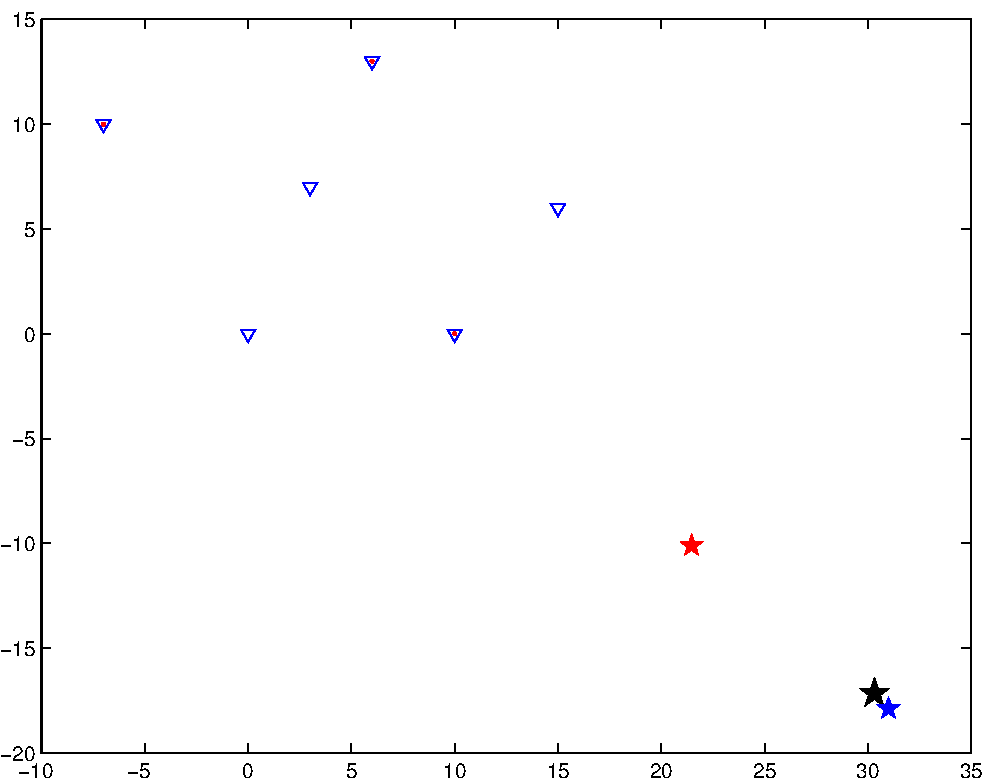
\includegraphics[width=10cm]{fig1.pdf}
  \caption{3(d): Location of earthquake in three cases. Black star, case 1; blue star, case 2; red star, case3.} 
\end{figure}

\lstinputlisting{hw3.m}




\end{document}